\documentclass[times, utf8, zavrsni]{fer}
\usepackage{booktabs}
\usepackage{listings}

\begin{document}

% TODO: Navedite broj rada.
\thesisnumber{797}

% TODO: Navedite naslov rada.
\title{Rješavanje problema bojanja grafa evolucijskim algoritmom}

% TODO: Navedite vaše ime i prezime.
\author{Filip Penzar}

\maketitle

% Ispis stranice s napomenom o umetanju izvornika rada. Uklonite naredbu \izvornik ako želite izbaciti tu stranicu.
% \izvornik

% Dodavanje zahvale ili prazne stranice. Ako ne želite dodati zahvalu, naredbu ostavite radi prazne stranice.
\zahvala{}

\tableofcontents

\chapter{Uvod}
Postoji mnogo NP-teških problema pretraživanja u kojima rješenje nije moguće pronaći iscrpnim pretraživanjem u realnom vremenu. Iz tog se razloga koriste heuristički algoritmi koji uz različite pretpostavke o problemu pronalaze rješenja u prihvatljivom vremenu, smanjujući prostor pretraživanja. Upravo zbog smanjivanja prostora pretraživanja rješenja pronađena takvim algoritmima nisu uvijek optimalna.

Jedan NP-težak problem je određivanje kromatskog broja grafa, a jedna heuristička skupina algoritama su evolucijski algoritmi. Ovaj rad pobliže opisuje način rada evolucijskih algoritama, njihov podskup genetskih algoritama, problem bojanja grafa, te primjenu i analizu evolucijskih algoritama pri određivanju kromatskog broja grafa.

U drugom poglavlju daje se kratko objašnjenje i uvod u problem određivanja kromatskog broja grafa. Zatim se u sljedećem poglavlju objašnjava princip rada evolucijskih algoritama te se detaljnije obrađuju genetski algoritmi, njihov način rada te različite varijacije parametara i funkcija koje utječu na kvalitetu dobivenog rješenja. U četvrtom poglavlju dan je kratak pregled korištenih biblioteka i podataka.

\chapter{Kromatski broj grafa}
\section{Uvod}
Kromatski broj grafa, $\chi(G)$, predstavlja minimalan broj boja s kojima se mogu obojati vrhovi grafa, tako da niti jedna dva susjedna vrha (vrhovi spojeni bridom) nisu obojana istom bojom. 

Kromatski broj koristi se u rješavanju mnogih problema; problema raspoređivanja, dodjele registara u procesoru, rješavanja Sudoku, dodjele radio frekvencije, sparivanje uzoraka, sinkronizacije paralelnih procesa itd. 

\begin{figure}[htb]
\centering
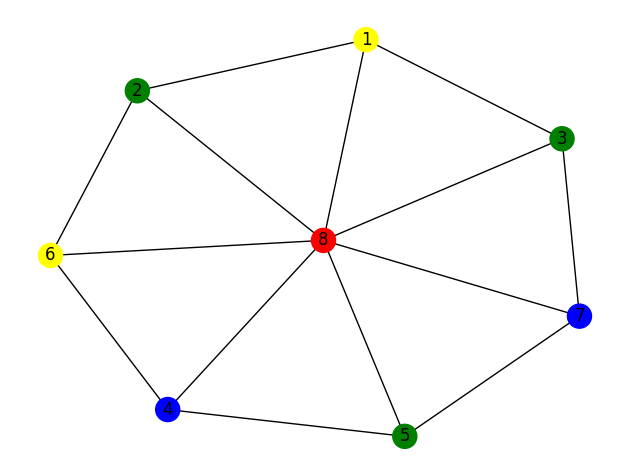
\includegraphics[width=10cm]{images/8_vertices_example.png}
\caption{Graf s osam vrhova i $\chi(G)=4$}
\label{fig:graf s obojanim vrhovima}
\end{figure}

\section{Određivanje kromatskog broja}
Pronalazak kromatskog broja grafa je NP-težak problem, što znači da je vremenska složenost njegovog pronalaska eksponencijalna. Zbog toga nije praktično koristiti se algoritmima iscrpnog pretraživanja na grafovima s većim brojem vrhova.

\subsection{Iscrpno pretraživanje}
Jednostavan algoritam isrcpnog pretreaživanja prošao bi sve kombinacije $k$ boja i $n$ vrhova; njegova vremenska složenost je $O(k^n)$. Implementacija iscrpnog algoritma određivanja kromatskog broja rekurzijom u programskom jeziku Python dana je slikom \ref{fig:algoritam iscrpnog pretraživanja}.

\begin{figure}[htb]
\centering
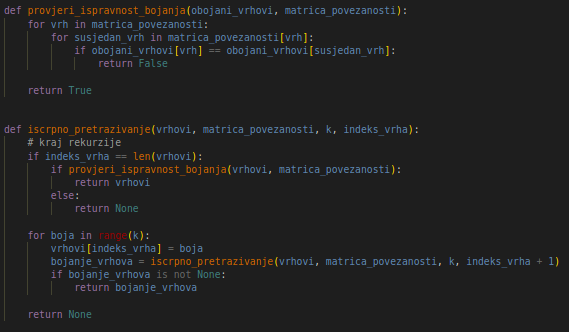
\includegraphics[width=12cm]{images/iscrpno_pretrazivanje.png}
\caption{Algoritam iscrpnog pretraživanja}
\label{fig:algoritam iscrpnog pretraživanja}
\end{figure}

Jedan iterativni pristup pronalaska kromatskog broja je pokušati obojati graf s $k=n$ boja, gdje je $n$ broj vrhova. Ukoliko uspijemo pronaći takvo rješenje, pokušavamo s $k=n-1$ bojom. Postupak nastavljamo sve do koraka $m: (m < n)$ kada više ne pronalazimo ispravno bojanje. Tada zaključujemo da je $\chi(G)=k=n-m+1$. Algoritam je prikazan slikom \ref{fig:algoritam iterativnog iscprnog odredivanja kromatskog broja}.

\begin{figure}[htb]
\centering
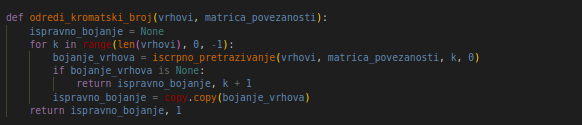
\includegraphics[width=12cm]{images/iterativni_algoritam_iscprnog_pretrazivanja.png}
\caption{Iterativno određivanje kromatskog broja s iscrpnim pretraživanjem}
\label{fig:algoritam iterativnog iscprnog odredivanja kromatskog broja}
\end{figure}

\subsection{Pohlepno pretraživanje}
Pohlepan algoritam kreće od vrha s najvećim stupnjem, onim s najviše susjednih vrhova. Njega boja prvom dostupnom bojom. Zatim pokušava obojati sljedeći vrh s najvećim stupnjem, uzimajući prvu boju s kojom može legalno obojati taj vrh, tako da je različite boje od njemu susjednih vrhova. Postupak se ponavlja do zadnjeg vrha, ili do kad više nema dostupnih boja. Složenost ovakvog algoritma je $O(n^2)$, jer za svaki vrh mora proći po svim dotad obojanim vrhovima i vidjeti kojim bojama može obojati trenutni vrh. Ovakvo pretraživanje ne daje uvijek rješenje kad ono postoji, no prednost mu je što je manje vremenske složenosti od iscrpnog pretraživanja. Algoritam je dan slikom \ref{fig:pohlepno pretrazivanje}.

\begin{figure}[htb]
\centering
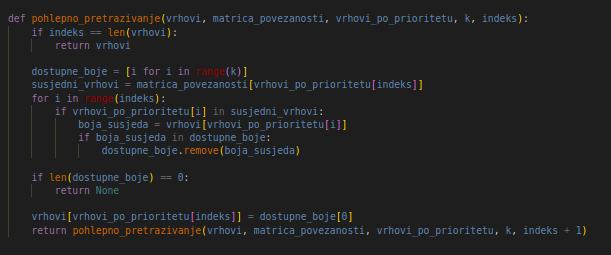
\includegraphics[width=12cm]{images/pohlepni_algoritam.png}
\caption{Pohlepno pretraživanje}
\label{fig:pohlepno pretrazivanje}
\end{figure}


\subsection{Usmjereno iscrpno pretraživanje}
Algoritam usmjerenog iscrpnog pretraživanja radi vrlo slično kao i pohlepno pretraživanje, uz bitnu preinaku da ukoliko ne pronađe legalno bojanje, traži dalje. Algoritam odredi moguće boje za bojanje trenutnog vrha kao i pohlepni algoritam, ali ukoliko ne uspije obojati graf s prvom bojom, proba s drugom mogućom, pa trećom i tako dalje. Ovakav će algoritam uvijek pronaći ispravno bojanje i upravo će to bojanje biti ono s minimalnim brojem boja, odnosno kromatski broj grafa. Algoritam je dan slikom \ref{fig:iscrpno usmjereno pretrazivanje}.

\begin{figure}[htb]
\centering
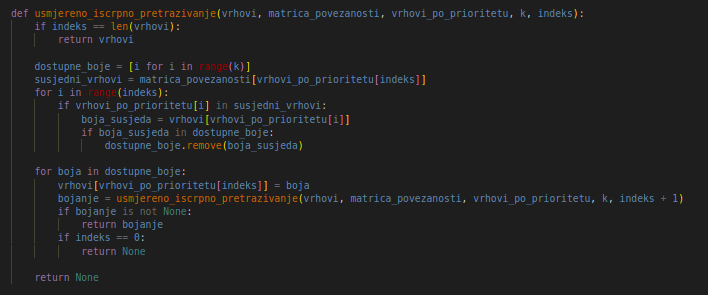
\includegraphics[width=12cm]{images/iscrpno_usmjereno_pretrazivanje.png}
\caption{Usmjereno iscrpno pretraživanje}
\label{fig:iscrpno usmjereno pretrazivanje}
\end{figure}

Svaki graf s $n$ vrhova možemo obojati s $n$ boja, no uvjet na gornju ogradu kromatskog broja možemo postrožiti.

\section{Gornja ograda na kromatski broj}
Prema Brookovom teoremu, kromatski broj svakog grafa je maksimalno $\Delta$ + 1, gdje je $\Delta$ maksimalan stupanj grafa. 

Maksimalan stupanj grafa, $\Delta$, je najveći broj bridova koji su incidentni s bilo kojim pojedinačnim vrhom u grafu.

\section{Donja ograda na kromatski broj}
Donja ograda na kromatski broj je 1. Ovo se postiže samo za grafove u kojima niti jedna dva vrha nisu međusobno povezana.

\begin{figure}[htb]
\centering
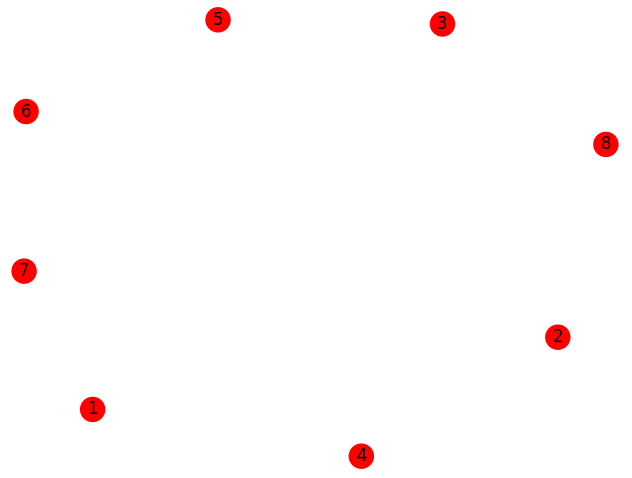
\includegraphics[width=10cm]{images/8_vertices_nepovezane.png}
\caption{Graf s $\chi(G)=1$}
\label{fig:graf s kromatskim brojem 1}
\end{figure}

\chapter{Evolucijski algoritmi}

Evolucijski algoritmi su algoritmi koji inspiraciju vuku iz prirode, iz Darwinonve teorije evolucije. Probleme rješavaju kroz procese koji emuliraju ponašanje živih bića i sustava u prirodi.

Rješenja problema u evolucijskim algoritmima predstavljaju pojedine jedinke unutar populacije. Populacija je na početku određena slučajno, a kasnije kroz naraštaje, odnosno iteracije algoritma, bolja rješenja preživljavaju i reproduciraju se, dok se lošija rješenja miču, izumiru. Ovime je osigurano da su jedinke novog naraštaja potomci najboljih jedinki prethodnog naraštaja čime se postiže konvergencija prema optimalnom rješenju.

Evolucijski algoritmi odlični su kod pronalaženja rješenja za optimizacijske probleme. Kroz naraštaje, pojedina rješenja postaju sve bolja i bliža optimalnom. Bitno je imati na umu da su evolucijski algoritmi podskup heurističkih algoritama, što znači da pronađena rješenja nisu nužno optimalna. Uzrok tome je što se ne pretražuje cijeli prostor već samo njegov podskup koji je ograničen početnom populacijom i parametrima evolucijskog algoritma, određenima na temelju neke heuristike.

\section{Genetski algoritmi}
Genetski algoritmi podskup su Evolucijskih algoritama. Jedinke, rješenja, kodirana su u obliku genoma. Iz početne populacije jedinki biraju se one najbolje pomoću funkcije dobrote (eng. \textit{fitness}) ili pomoću funkcije cijene (eng. \textit{cost}) koje će biti roditelji novoj generacije. Iz genoma odabranih roditelja se pomoću procesa križanja određuju genomi djece. Osim procesa križanja i odabira roditelja, važnu ulogu igraju i mutacije gena na genomu. Proces mutacije događa se nakon križanja roditelja, kada se s određenom vjerojatnošću ili heuristikom mijenjaju neki od gena na genomu. Mutacije su bitne jer se njima proširuje prostor pretraživanja, uvode nove varijacije rješenja te se sprječava ostanak u području lokalnog optimuma rješenja.

\subsection{Kodiranje genoma}
Genom (kromosom) u sklopu Genetskih algoritama predstavlja jedan specifičan organizam, odnosno jedno moguće rješenje. Genom se sastoji od vektora gena. Svaki gen može poprimiti određenu vrijednost. Za ispravan rad genetskog algoritma nužno je pravilno kodirati rješenja u obliku genoma.

Kod problema bojanja grafa, genom je vektor od $n$ elemenata gdje je $n$ broj vrhova u grafu. Vrijednost svakog gena je iz skupa od $k$ elemenata, gdje $k$ predstavlja broj različitih boja. Konačno rješenje je vektor u kojemu su elementi pobojani s $k$ različitih boja tako da pripadajući spojeni vrhovi nemaju istu vrijednost. Ukoliko su dva vrha spojena i obojana su istom bojom, takvu jedniku ne smatramo rješenjem problema. Na slici \ref{fig:kodirani genom} prikazan je genom jedne jedinke koja je optimalno rješenje bojanja grafa na slici \ref{fig:kodiranje genoma graf}.

\begin{figure}[htb]
\centering
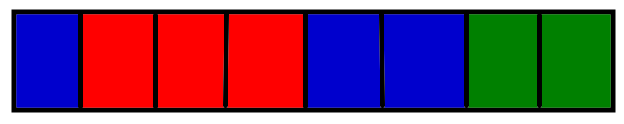
\includegraphics[width=8cm]{images/genom_encoding.png}
\caption{Vektor gena - genom, $k=3$, $n=8$}
\label{fig:kodirani genom}
\end{figure}

\begin{figure}[htb]
\centering
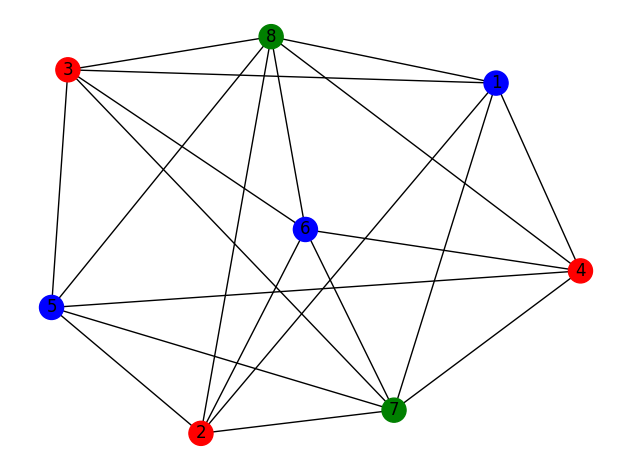
\includegraphics[width=10cm]{images/genom_encoding_graph.png}
\caption{Pripadajući obojani graf, $\chi(G)=3$}
\label{fig:kodiranje genoma graf}
\end{figure}

\subsection{Funkcija cijene}
Određivanje koliko je koja jedinka dobra određuje se pomoću funkcije cijene. Ona mjeri koliko je trenutno rješenje udaljeno od ciljnog. Što je cijena jedinke manja, to je rješenje bolje. Kada cijene neke jedinke dosegne 0, pronađeno je ispravno rješenje.

Suprotno funkciji cijene je funkcija dobrote, prema kojoj bolje jedinke imaju veću vrijednost.

U primjeru bojanja grafova, ciljno rješenje ne smije imati niti jedna dva susjedna vrha obojana istom bojom. Za svaka dva krivo spojena vrha, funkcija cijene raste za jedan. Implementacija algoritma prikazana je slikom \ref{fig:funkcija cijene}.

\begin{figure}[htb]
\centering
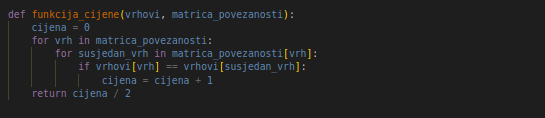
\includegraphics[width=12cm]{images/funkcija_cijene.png}
\caption{Funkcija cijene implementirana u Pythonu}
\label{fig:funkcija cijene}
\end{figure}

\subsection{Određivanje roditelja}
Roditelji se iz populacije biraju na temelju njihove izračunate cijene. Jedinke s manjom cijenom imaju prednost pri reproduciranju nad jedinkama s većom cijenom. Postoji mnogo različitih načina odabira roditelja u sklopu genetskih algoritama, no ovaj projekt se zadržao na sljedeća tri:
\begin{itemize}
    \item Slučajna selekcija
    \item Roullete wheel
    \item Rang selekcija
\end{itemize}

\subsubsection{Slučajna selekcija}
Kao naivnu metodu selekcije roditelja koristi se Slučajna selekcija. Iz populacije se slučajnim odabirom izabiru dvije jedinke kao roditelji novoj jedinci. Ova metoda je manje uspješna od ostalih metoda selekcije i zato nije pretjerano korištena. Razlog manjoj uspješnosti je što cijena izračunata za pojedine jedinke nimalo ne utječe na izbor jedinke kao roditelja. Bolje jedinke nemaju nikakvu prednost kod reprodukcije što znači da rješenja sporije konvergiraju, ili uopće ne konvergiraju k optimumu.

\subsubsection{Roullete wheel}
Nakon što su izračunate cijene za sve jedinke u generaciji, svakoj se pridjeljuje udio na \textit{roullete wheel-u}. Udio je proporcionalan cijenama jedinki; one s nižom cijenom (većom dobrotom) će imati veći udio na \textit{roullete wheel-u}. Time se osigurava da bolje jedinke imaju veću vjerojatnost da budu odabrane kao roditelji sljedećoj generaciji. Rješenje se tako brže približava optimumu jer će djeca naslijediti gene od uspješnijih roditelja. 

\begin{figure}[htb]
\centering
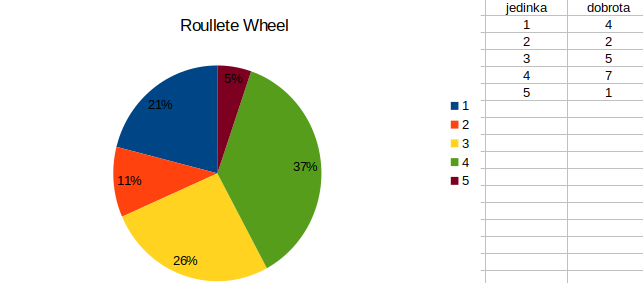
\includegraphics[width=14cm]{images/roullete_wheel_selection.png}
\caption{Primjer \textit{roullete wheel-a}}
\label{fig:roullete wheel}
\end{figure}

Nedostatak ove metode je što se može dogoditi da neka jedinka bude nesrazmjerno dobra u odnosu na druge jedinke, ali vodi samo lokalnom optimumu. Algoritam će tada odabrati takvu jedinku kao roditelja i sva njezina djeca će posljedično biti relativno uspješna, ali neće konvergirati optimalnom rješenju.

\subsubsection{Rang selekcija}
Rang selekcija po principu je slična \textit{roullete wheel-u}, ali se umjesto proporcionalnog udjela vjerojatnosti prema cijeni, jedinke prvo rangiraju prema cijeni, a udjeli na kotaču se zatim dodjeljuju proporcionalno rangu.

\begin{figure}[htb]
\centering
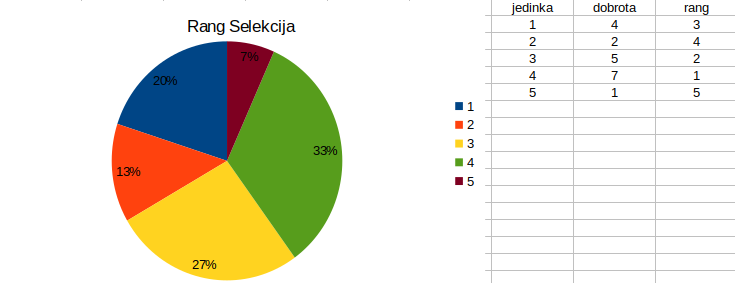
\includegraphics[width=14cm]{images/rang_selekcija.png}
\caption{Primjer rang selekcije}
\label{fig:rang selekcija}
\end{figure}

Na taj način svaki rang uvijek ima jednaku vjerojatnost biti izabran. Bolje jedinke imaju veću vjerojatnost biti izabrane kao roditelji sljedećoj generaciji, a ne može se dogoditi da neke jedinke koje vode do lokalnog optimuma imaju preveliku prednost nad ostalim jedinkama te da zbog toga algoritam ne konvergira u globalno rješenje.

\subsection{Križanje}
Križanje je postupak kojim se iz izabranih genoma roditelja dobiva genom potomka. Potomak se sastoji od pomješanog genoma svojih roditelja. Križanje se izvodi tako da se na slučajnom mjestu prerežu genomi oba roditelja u točki prijeloma, zamijene se prvi dijelovi genoma i dobiju se dvije nove jedinke; prva jedinka s prvim dijelom genoma od prvog roditelja i drugim dijelom genoma od drugog roditelja, i druga jedinka s prvim dijelom genoma od drugog roditelja i drugim dijelom genoma od prvog roditelja.

Postupak križanja vizualno je prikazan na slikama \ref{fig:kromosomi roditelja}, \ref{fig:krizanje}, \ref{fig:kromosomi djece}.

\begin{figure}[htb]
\centering
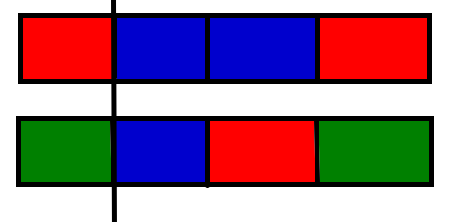
\includegraphics[width=4cm]{images/kromosomi_roditelja.png}
\caption{Kromosomi roditelja}
\label{fig:kromosomi roditelja}
\end{figure}

\begin{figure}[htb]
\centering
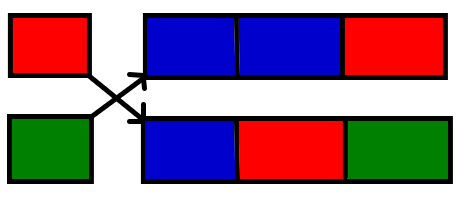
\includegraphics[width=4cm]{images/krizanje.png}
\caption{Križanje}
\label{fig:krizanje}
\end{figure}

\begin{figure}[htb]
\centering
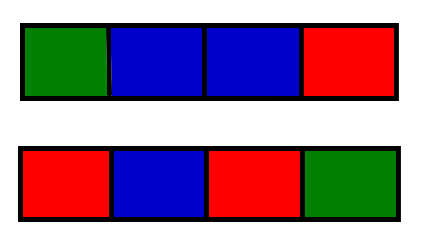
\includegraphics[width=4cm]{images/kromosomi_djece.png}
\caption{Kromosomi djece}
\label{fig:kromosomi djece}
\end{figure}

Ukoliko smo koristili dobru metodu za odabir roditelja, djeca će se sastojati od pomiješanih gena uspješnih roditelja, približiti će se optimumu. Često se dogodi da su djeca manje dobrote od svojih roditelja, no prosječno gledano na cijeloj populaciji, dobrota djece se povećava.

\subsection{Mutacije}
Mutacije su promjene gena na kromosomima jedinki. One su vrlo bitne u genetskim algoritmima jer nam omogućuju da pretražujemo rješenje na širem prostoru. Ukoliko ne bismo uveli mutacije na genima, geni početne populacije bi u potpunosti određivali mogući prostor pretraživanja. Sve nove jedinke mogle bi biti jedino kombinacije početnog skupa gena. Mutacije također ubrazavaju pretraživanje prostora, jer će neke jedinke "odskočiti" od trenutne populacije, uvesti novinu u naš skup jedinki. Ukoliko su mutacije nepovoljne, takve jedinke imati će manju dobrotu, neće se uspješno razmnožavati i takva mutacija će izumrijeti. Pozitivne će mutacije s druge strane, povećati dobrotu jedinke i tako povećati vjerojatnost reprodukcije jedinke s takvim genom. Gen će se dalje propagirati i dovesti cijelu populaciju bliže optimumu.

Slika \ref{fig:kromosom prije mutacije} prikazuje kromosom prije mutacije, a slika \ref{fig:kromosom poslije mutacije} kromosom poslije mutacije na trećem i osmom genu.

\begin{figure}[htb]
\centering
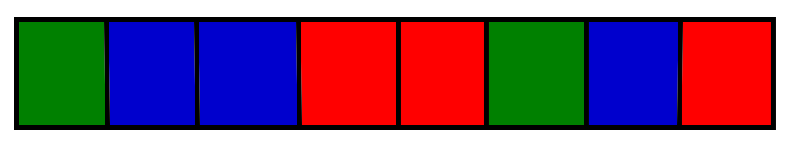
\includegraphics[width=4cm]{images/prije_mutacije.png}
\caption{Kromosom prije mutacije}
\label{fig:kromosom prije mutacije}
\end{figure}

\begin{figure}[htb]
\centering
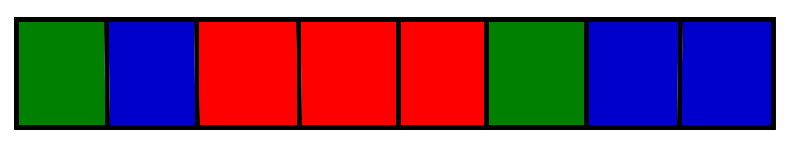
\includegraphics[width=4cm]{images/poslije_mutacije.png}
\caption{Kromosom poslije mutacije}
\label{fig:kromosom poslije mutacije}
\end{figure}

Klasično se mutacije implementiraju tako da svaki gen ima nezavisnu vjerojatnost mutacije. Mutacija se provodi nakon križanja. Kod nekih specifičnih problema, poput bojanja grafa, bolje rezultate daju usmjere mutacije na genima koje ovise o trenutnom stanju svih gena jedinke.

\section{Implementacija genetskog algoritma}
Nakon slučajnog izbora početne populacije, nad svakom jedinkom izračunava se njezina dobrota. Na temelju dobrote se odabiru roditelji nove generacije. Roditelji se križaju, a zatim se nad dobivenom djecom izvode mutacije. Djeca zamjenjuju roditelje u populaciji. Ovaj se postupak ponavlja sve dok se ne postigne željena dobrota, pronađe optimalno rješenje problema, ili se ne pređe određen broj iteracija. Pseudokod genetskog algoritma dan je slikom \ref{fig:pseudokod genetskog algoritma}.

\begin{figure}[htb]
\centering
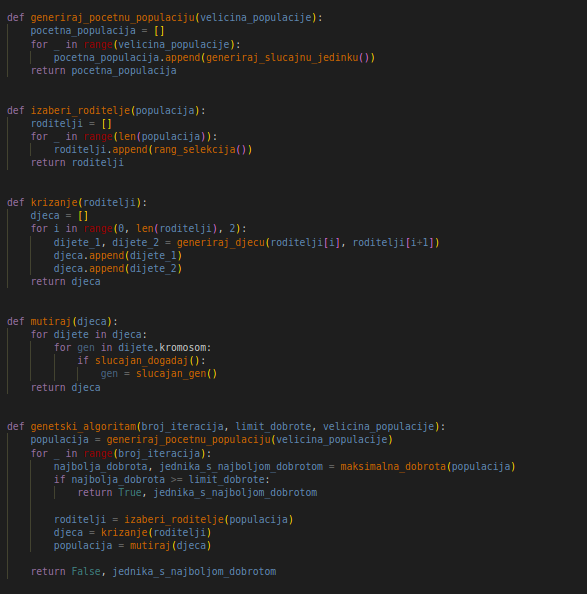
\includegraphics[width=14cm]{images/genetski_algoritam_pseudokod.png}
\caption{Pseudokod genetskog algoritma}
\label{fig:pseudokod genetskog algoritma}
\end{figure}

\chapter{Korištene biblioteke i podaci}
Projekt je pisan u programskom jeziku Python koristeći slobodno dostupne biblioteke.

\section{PyGAD}
PyGAD je biblioteka otvorenog koda za programski jezik Python pomoću koje se vrlo jednostavno mogu izgraditi modeli genetskih algoritama. Biblioteka dolazi s mnoštvom ugrađenih metoda, specifičnima za genetske algoritme. PyGAD je vrlo fleksibilan i dozvoljava definiranje vlastitih funckija izračuna dobrote, izbora roditelja, križanja i mutacije.

\subsection{Instalacija}
Instalacija biblioteke vrši se preko PIP-a sljedećom naredbom:

\begin{lstlisting}[language=bash]
  $ pip install pygad
\end{lstlisting}

\section{NetworkX}
NetworkX je Python paket za stvaranje, rukovanje i proučavanje strukture, dinamike i funkcija složenih mreža. U sklopu ovog projekta korišten je kod vizualizacije grafova te njihovog bojanja.

\subsection{Instalacija}
Instalacija biblioteke vrši se preko PIP-a sljedećom naredbom:

\begin{lstlisting}[language=bash]
  $ pip install networkx[default]
\end{lstlisting}

\section{House of Graphs}
House of Graphs je Web-stranica koja sadržava bazu grafova s karakteristikama koja dozvoljava njihovo besplatno preuzimanje. House of Graphs razvijen je u suradnji sveučilišta Ghent i sveučilišta KU Leuven.

U sklopu projekta preuzeti su grafovi s brojem vrhova između 1 i 250. Za svaki od grafova definirana je matrica susjedstva kao i kromatski broj grafa. Na taj se način rješenje dobiveno genetskim algoritmom može usporediti sa stvarnom vrijednošću kromatskog broja grafa. Za neke od kompleksnijh grafova nije izračunat kromatski broj (\textit{Chromatic number: Computation timeout}) te su takvi grafovi preskočeni kod izračuna točnosti rada genetskog algoritma.

\begin{figure}[h]
\centering
\begin{minipage}{.5\textwidth}
  \centering
  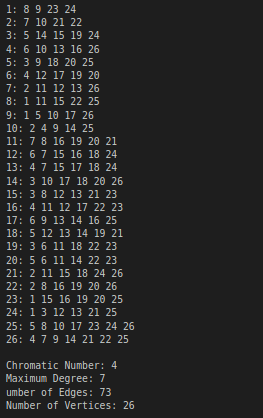
\includegraphics[width=5cm]{images/26_vertices_graph_definition.png}
  \caption{Definicija grafa s 26 vrhova}
  \label{fig:definicija grafa s 26 vrhova}
\end{minipage}%
\begin{minipage}{.5\textwidth}
  \centering
  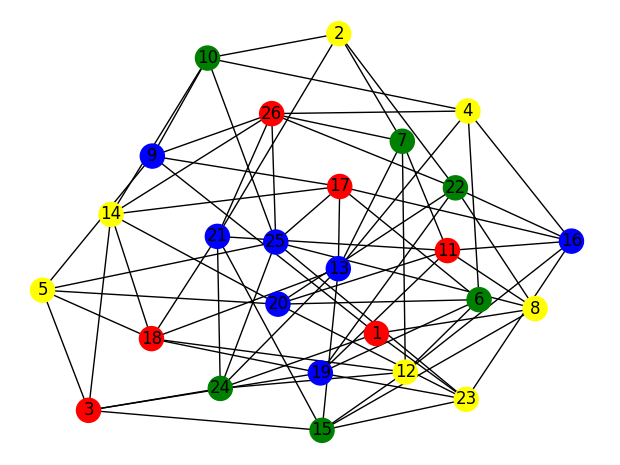
\includegraphics[width=8cm]{images/26_vertices_graph.png}
  \caption{Bojanje grafa s 26 vrhova s 4 boje}
  \label{fig:obojani graf s 26 vrhova}
\end{minipage}
\end{figure}

Definicija grafa preuzetog s House of Graphs Web-stranice s 26 vrhova dana je slikom \ref{fig:definicija grafa s 26 vrhova}, a ispravno bojanje za taj graf dano je slikom \ref{fig:obojani graf s 26 vrhova}.


\chapter{Praktični dio}

\chapter{Rezultati praktičnog dijela}

\chapter{Zaključak}
Zaključak.

\bibliography{literatura}
\bibliographystyle{fer}

\begin{sazetak}
Sažetak na hrvatskom jeziku.

\kljucnerijeci{Ključne riječi, odvojene zarezima.}
\end{sazetak}

% TODO: Navedite naslov na engleskom jeziku.
\engtitle{Solving graph coloring problem using evolutionary algorithm}
\begin{abstract}
Abstract.

\keywords{Keywords.}
\end{abstract}

\end{document}

